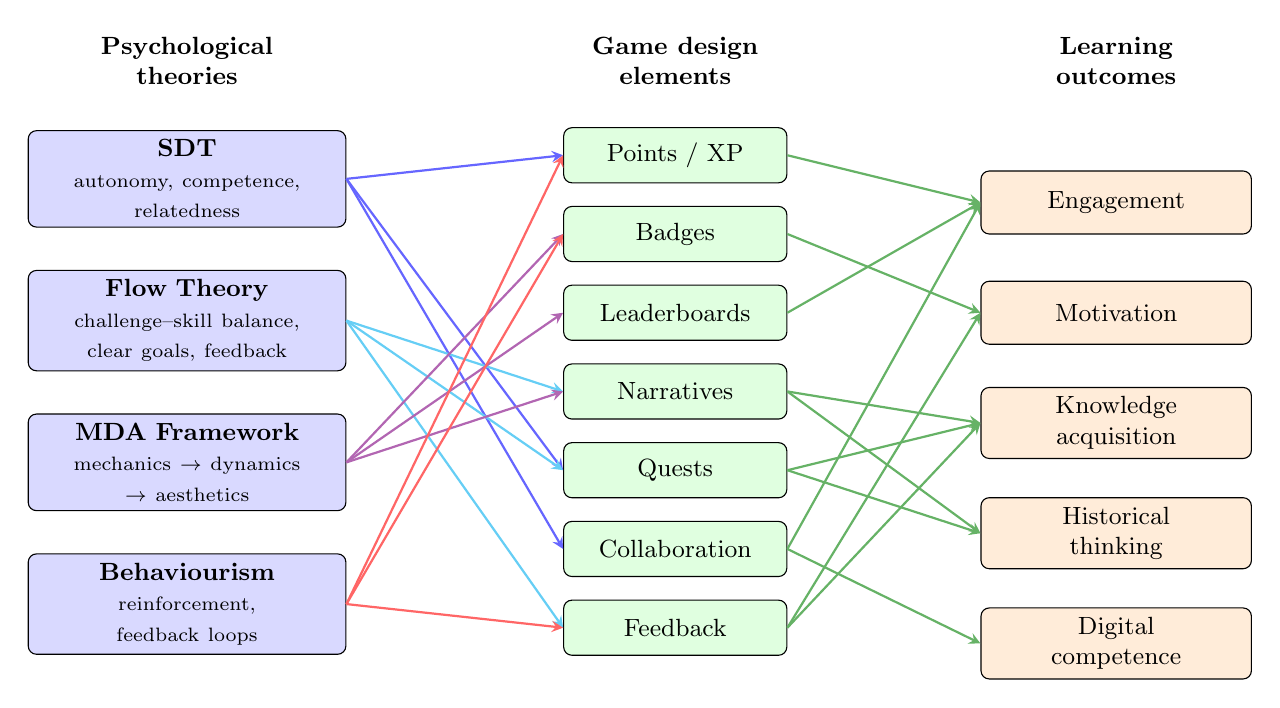
\begin{tikzpicture}[
  node distance=0.5cm,
  theorybox/.style={rectangle, draw, rounded corners=3pt, fill=#1!15,
    text width=3.8cm, minimum height=1cm, align=center, font=\small},
  theorybox/.default=blue,
  elembox/.style={rectangle, draw, rounded corners=3pt, fill=green!12,
    text width=2.6cm, minimum height=0.7cm, align=center, font=\small},
  outbox/.style={rectangle, draw, rounded corners=3pt, fill=orange!15,
    text width=3.2cm, minimum height=0.8cm, align=center, font=\small},
  colhead/.style={font=\bfseries\small, align=center},
  arr/.style={->, >=stealth, thick, #1!60},
  arr/.default=gray
]

% Column headers
\node[colhead] (h1) at (0, 0) {Psychological\\theories};
\node[colhead] (h2) at (6.2, 0) {Game design\\elements};
\node[colhead] (h3) at (11.8, 0) {Learning\\outcomes};

% Column 1: Theories
\node[theorybox=blue] (sdt) at (0, -1.5) {\textbf{SDT}\\{\scriptsize autonomy, competence,}\\{\scriptsize relatedness}};
\node[theorybox=blue] (flow) at (0, -3.3) {\textbf{Flow Theory}\\{\scriptsize challenge--skill balance,}\\{\scriptsize clear goals, feedback}};
\node[theorybox=blue] (mda) at (0, -5.1) {\textbf{MDA Framework}\\{\scriptsize mechanics $\to$ dynamics}\\{\scriptsize $\to$ aesthetics}};
\node[theorybox=blue] (behav) at (0, -6.9) {\textbf{Behaviourism}\\{\scriptsize reinforcement,}\\{\scriptsize feedback loops}};

% Column 2: Game elements
\node[elembox] (points) at (6.2, -1.2) {Points / XP};
\node[elembox] (badges) at (6.2, -2.2) {Badges};
\node[elembox] (leader) at (6.2, -3.2) {Leaderboards};
\node[elembox] (narr) at (6.2, -4.2) {Narratives};
\node[elembox] (quests) at (6.2, -5.2) {Quests};
\node[elembox] (collab) at (6.2, -6.2) {Collaboration};
\node[elembox] (feedb) at (6.2, -7.2) {Feedback};

% Column 3: Outcomes
\node[outbox] (engage) at (11.8, -1.8) {Engagement};
\node[outbox] (motiv) at (11.8, -3.2) {Motivation};
\node[outbox] (knowl) at (11.8, -4.6) {Knowledge\\acquisition};
\node[outbox] (hist) at (11.8, -6.0) {Historical\\thinking};
\node[outbox] (digcomp) at (11.8, -7.4) {Digital\\competence};

% Arrows: SDT → elements (competence, autonomy, relatedness)
\draw[arr=blue] (sdt.east) -- (points.west);
\draw[arr=blue] (sdt.east) -- (quests.west);
\draw[arr=blue] (sdt.east) -- (collab.west);

% Arrows: Flow → elements
\draw[arr=cyan] (flow.east) -- (narr.west);
\draw[arr=cyan] (flow.east) -- (quests.west);
\draw[arr=cyan] (flow.east) -- (feedb.west);

% Arrows: MDA → elements
\draw[arr=violet] (mda.east) -- (narr.west);
\draw[arr=violet] (mda.east) -- (badges.west);
\draw[arr=violet] (mda.east) -- (leader.west);

% Arrows: Behaviourism → elements
\draw[arr=red] (behav.east) -- (points.west);
\draw[arr=red] (behav.east) -- (badges.west);
\draw[arr=red] (behav.east) -- (feedb.west);

% Arrows: elements → outcomes
\draw[arr=green!50!black] (points.east) -- (engage.west);
\draw[arr=green!50!black] (badges.east) -- (motiv.west);
\draw[arr=green!50!black] (leader.east) -- (engage.west);
\draw[arr=green!50!black] (narr.east) -- (hist.west);
\draw[arr=green!50!black] (quests.east) -- (knowl.west);
\draw[arr=green!50!black] (collab.east) -- (digcomp.west);
\draw[arr=green!50!black] (feedb.east) -- (motiv.west);
\draw[arr=green!50!black] (narr.east) -- (knowl.west);
\draw[arr=green!50!black] (quests.east) -- (hist.west);
\draw[arr=green!50!black] (collab.east) -- (engage.west);
\draw[arr=green!50!black] (feedb.east) -- (knowl.west);

\end{tikzpicture}
